\documentclass[11pt,sigconf,nonacm]{acmart}

\usepackage{booktabs}
\usepackage{graphicx}

\setlength{\emergencystretch}{3em}

\settopmatter{printacmref=false}
\renewcommand\footnotetextcopyrightpermission[1]{}
\pagestyle{plain}

\title{Predicting Steam Game Popularity from Storefront Metadata}

\author{Terry Su}
\affiliation{
  \institution{University of California San Diego}
  \city{La Jolla}
  \state{California}
  \country{USA}
}
\email{t9su@ucsd.edu}

\author{Kyle Zhao}
\affiliation{
  \institution{University of California San Diego}
  \city{La Jolla}
  \state{California}
  \country{USA}
}
\email{kyzhao@ucsd.edu}

\begin{abstract}
This project studies whether Steam game popularity can be predicted from launch-visible storefront metadata. Using the March 2025 cleaned Steam Games Dataset, we define a binary task: predict whether a game falls in the top quartile of total review count among games released in the same year. We avoid leakage by excluding owner estimates, reviews, review scores, playtime, peak concurrent users, recommendations, Metacritic fields, and other post-release engagement variables from the input features. Our best model is a leakage-cleaned linear classifier using price, platform, release timing, and store metadata such as genres, tags, categories, supported languages, developers, and publishers. On a temporal split that trains on 2009--2022 releases and tests on 2023--2025 releases, this model reaches PR-AUC 0.612 and ROC-AUC 0.804, substantially above the majority baseline PR-AUC of 0.251. Description text alone is weaker, and an SVD plus histogram gradient boosting model does not outperform the sparse linear metadata model.
\end{abstract}

\keywords{Steam, game popularity, classification, text mining, data leakage, TF-IDF}

\begin{document}

\maketitle

\section{Introduction}

Steam contains a large and rapidly growing catalog of games, making discoverability and commercial success difficult to predict. Developers, publishers, and platform designers may want to estimate whether a game has traits associated with high post-release attention before large-scale launch investment. We frame this as a data mining problem: given launch-visible Steam store metadata, predict whether a game will be relatively popular within its release-year cohort.

The central challenge is target leakage. Steam datasets often include review counts, owner estimates, recommendations, playtime, and concurrent-user fields. These are strong measures of popularity, but they are not launch-time features. This project therefore uses post-release review count only to define the target, while excluding review-derived and engagement-derived columns from the feature matrix. This setup makes the task harder, but it better matches the realistic question of whether metadata available around launch can forecast later attention.

Our contributions are threefold. First, we construct a leakage-aware popularity prediction task from a large 2025 Steam dataset. Second, we compare linear baselines, feature ablations, and a non-linear reduced-dimensionality model using a temporal split. Third, we analyze errors to identify which kinds of games are over- or under-predicted by launch-visible metadata.

\section{Related Work}

Prior work motivates both our task and our modeling choices. De Luisa et al. study Steam popularity prediction from features such as price, supported languages, release timing, and genres, using a Bayesian approach to understand how early game features relate to player counts \citep{deluisa2021steam}. Their framing is close to ours, but we emphasize a large 2025 snapshot, a top-quartile classification target, and explicit leakage removal.

Vu and Bezemer examine discoverability by comparing indie games to top-selling games \citep{vu2021discoverability}. Their work supports the intuition that tags, genres, and content similarity can provide useful signals about future attention. Ma studies broader success drivers across Steam, Twitch, and Metacritic \citep{ma2025success}. That work shows that community and platform metrics can be strongly predictive, but it also motivates our leakage boundary: those signals are useful after release but should not be used as launch-time predictors.

For modeling, gradient-boosted decision trees are a common choice for structured prediction tasks. XGBoost \citep{chen2016xgboost} and LightGBM \citep{ke2017lightgbm} motivate scalable tree-based methods for sparse and high-dimensional data. A related Steam rating regression study also compares machine-learning approaches on Steam metadata \citep{teja2023rating}. In our experiments, however, sparse linear models are more effective than a compressed non-linear model, which suggests that preserving high-dimensional tag and metadata indicators matters for this task.

\section{Dataset and Exploratory Analysis}

We use \texttt{games\_march2025\_cleaned.csv} from the Steam Games Dataset 2025 \citep{kaggle_steam_2025}. The cleaned CSV contains 89,618 rows and 47 columns with no duplicate rows. Important fields include \texttt{name}, \texttt{release\_date}, \texttt{price}, platform flags, descriptions, supported languages, developers, publishers, categories, genres, tags, review counts, owner estimates, playtime, and peak concurrent users.

The dataset is highly skewed. Review activity and owner estimates follow a long-tail distribution where a small number of games receive extremely high attention. Genre and tag frequencies are also imbalanced: common labels such as Indie, Casual, Action, Adventure, Simulation, Strategy, and RPG dominate. Missingness varies substantially across columns; for example, Metacritic URL and editorial reviews are mostly missing, while core store metadata is much more complete.

\begin{figure}[t]
  \centering
  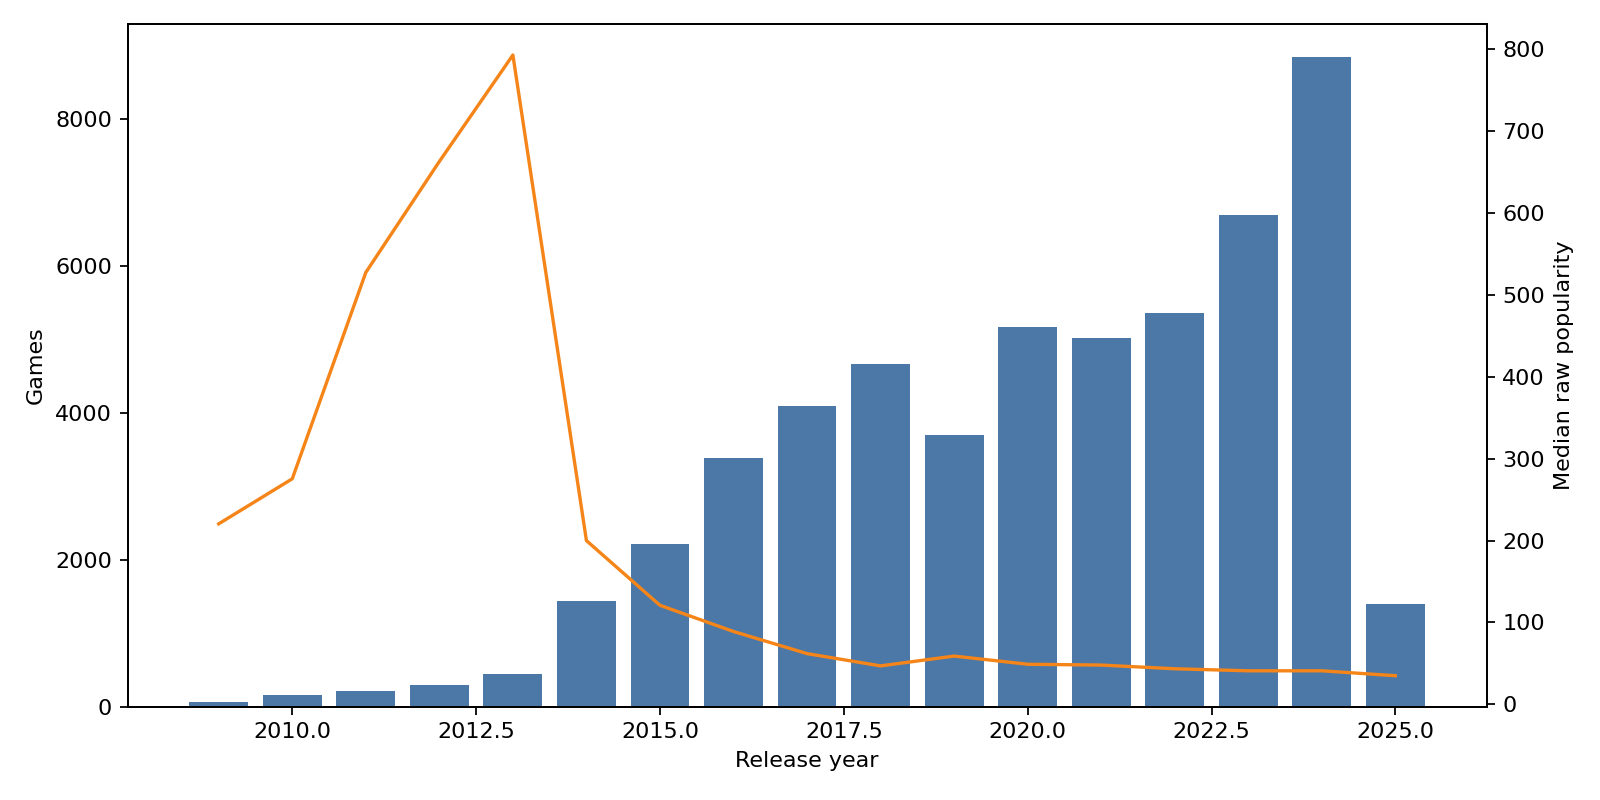
\includegraphics[width=\linewidth]{figures/games_and_popularity_by_year.png}
  \caption{Number of games and median raw popularity by release year after target construction. The growth in yearly releases makes cohort-normalized labels preferable to a single global threshold.}
  \Description{Bar chart of number of games by year with a line for median popularity. Recent release years contain many more games.}
  \label{fig:yearly}
\end{figure}

\begin{figure}[t]
  \centering
  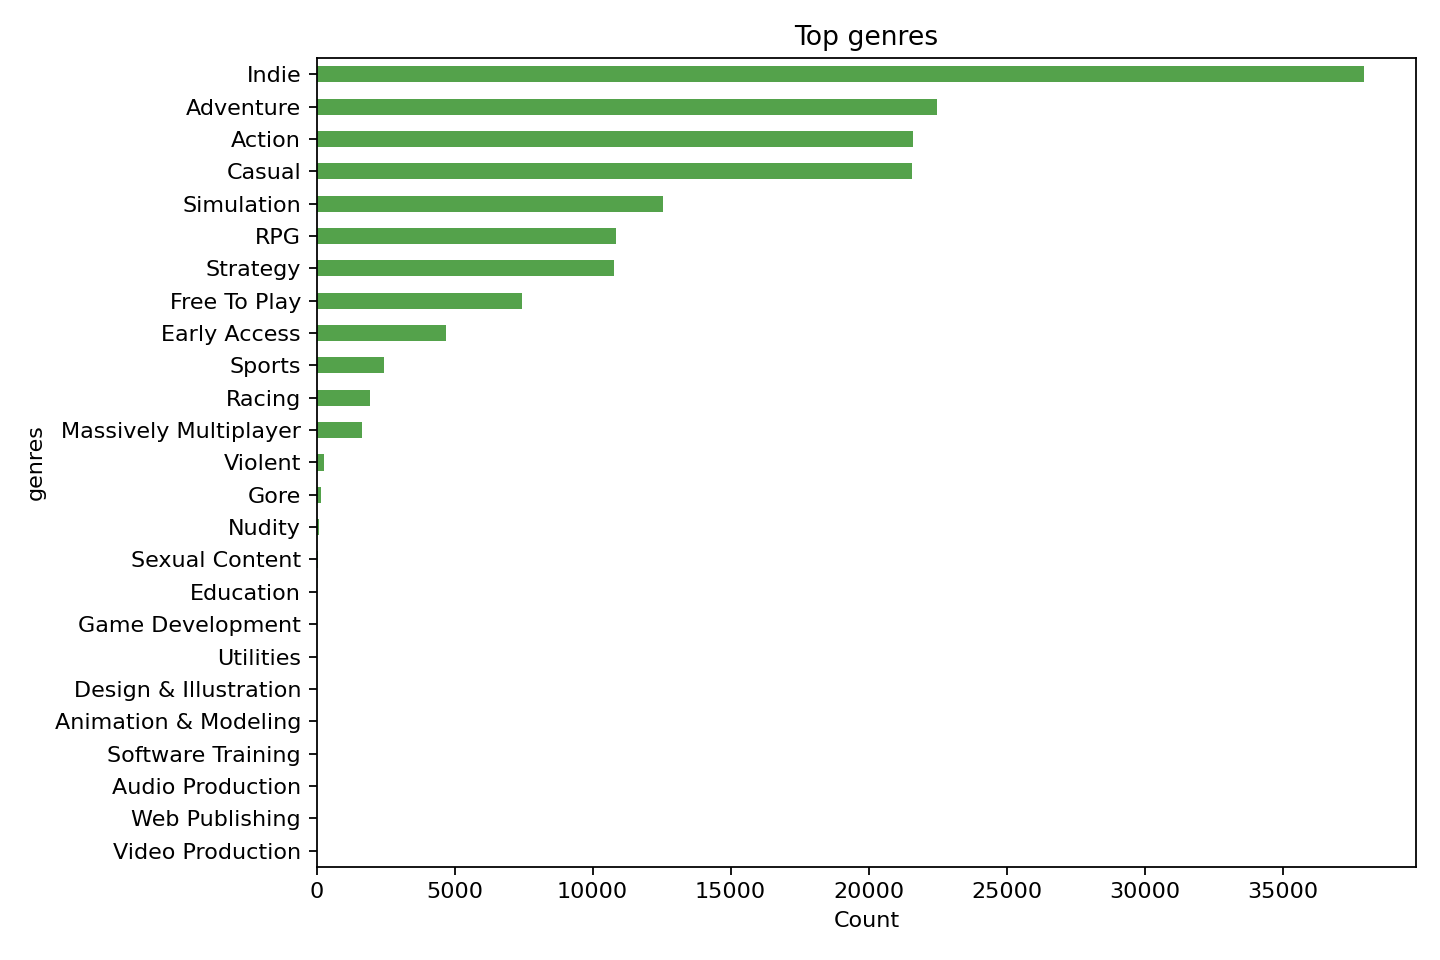
\includegraphics[width=\linewidth]{figures/top_genres.png}
  \caption{Most frequent genre labels in the cleaned Steam dataset. Common tags such as Indie, Casual, Action, and Adventure dominate the catalog.}
  \Description{Horizontal bar chart showing Indie, Casual, Action, and Adventure as the most frequent genres.}
  \label{fig:genres}
\end{figure}

\begin{figure}[t]
  \centering
  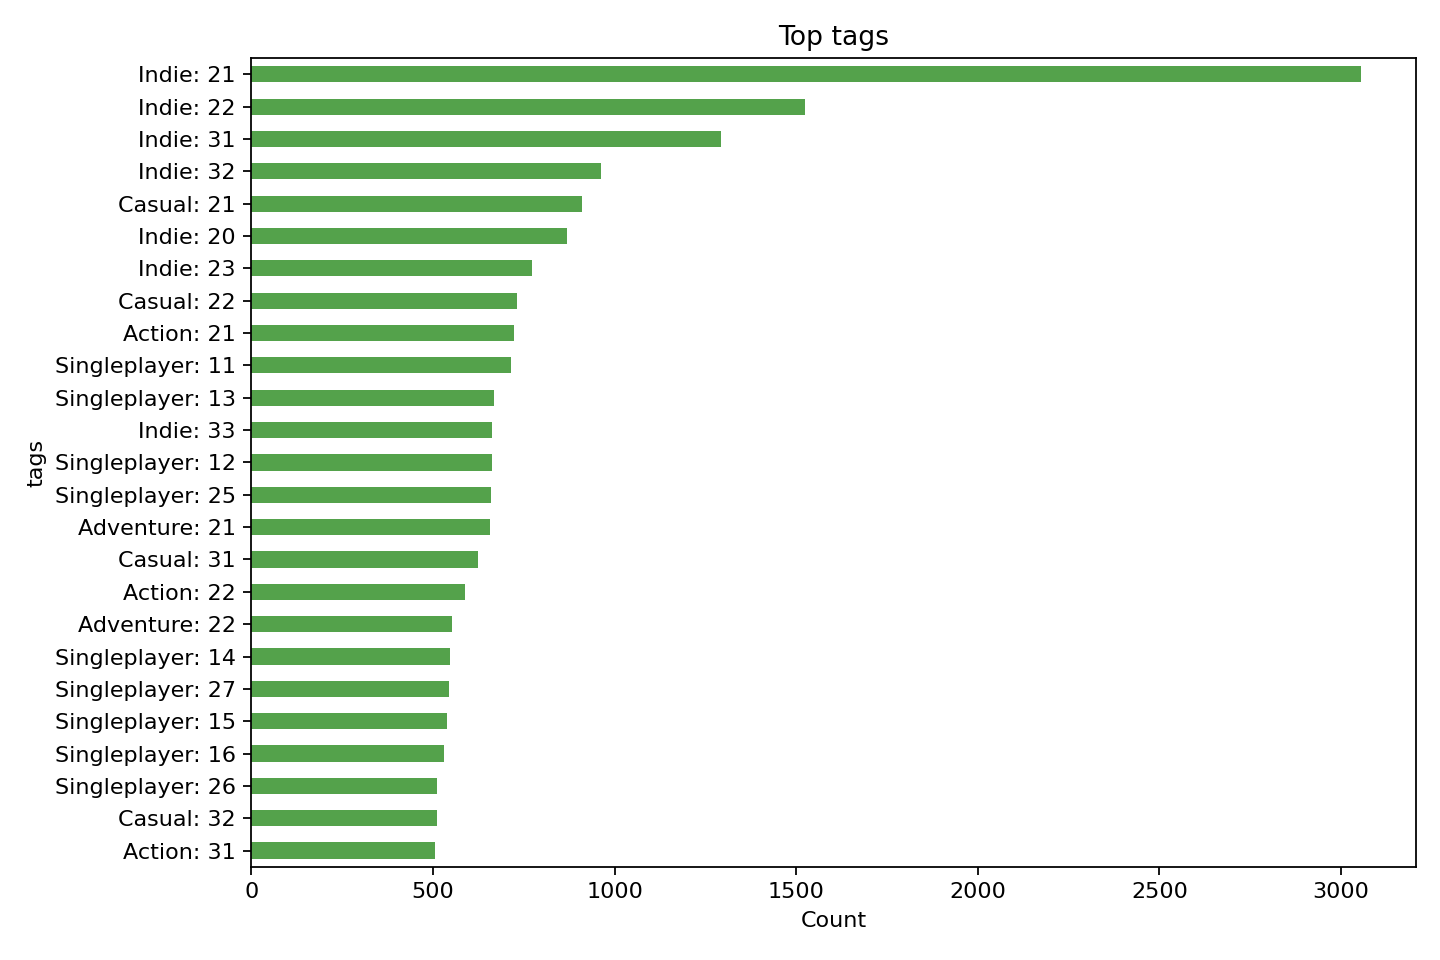
\includegraphics[width=\linewidth]{figures/top_tags.png}
  \caption{Most frequent user tags. Tags provide a richer description of gameplay style than broad genre labels, which helps explain their strong ablation performance.}
  \Description{Horizontal bar chart of common Steam tags such as Singleplayer, Indie, Adventure, Action, and Casual.}
  \label{fig:tags}
\end{figure}

We initially considered \texttt{estimated\_owners} as the popularity target, but it is too coarse for this classification task. It has only 14 unique buckets and creates excessive ties, especially in recent years. In contrast, \texttt{num\_reviews\_total} has thousands of unique values and produces a stable within-year top-quartile class. We therefore use total review count as the post-release popularity proxy.

Several additional EDA findings shaped the final model design. First, the number of releases increases sharply in recent years, which makes a temporal split more realistic than a random split. Second, many columns that look predictive are actually post-release outcomes: owner estimates, playtime, review ratios, recent review counts, and peak CCU are all highly related to popularity but unavailable at launch. Third, descriptive fields vary widely in length and quality. Some games include detailed descriptions, while others use short boilerplate text. This suggested that description text should be evaluated separately rather than assumed useful.

\section{Predictive Task}

For each game, we define the binary label
\[
popular_i =
\begin{cases}
1, & r_i \ge Q_{0.75}(R_{y_i}) \\
0, & \text{otherwise,}
\end{cases}
\]
where $r_i$ is the game's total review count, $y_i$ is its release year, and $Q_{0.75}(R_{y_i})$ is the 75th percentile review count among games released in year $y_i$. This cohort-normalized target reduces the bias that older games have had more time to accumulate reviews.

Games with invalid review-count sentinels are dropped. The final labeled dataset contains 53,162 games with a positive rate of 25.05\%. We use a temporal split: training data contains games released from 2009 through 2022, and test data contains games released from 2023 through 2025. This split is stricter than a random split because it evaluates whether patterns learned from older Steam releases transfer to newer releases.

Primary metrics are PR-AUC and ROC-AUC. PR-AUC is especially important because only one quarter of games are labeled popular. We also report accuracy, precision, recall, and F1.

The task intentionally predicts relative attention, not absolute commercial success. Review count is only a proxy for popularity: a game can sell many copies with relatively few reviews, and review behavior can vary by genre and audience. However, total reviews are more fine-grained than Steam Spy owner buckets in this dataset, making them more suitable for constructing stable labels.

\section{Models and Features}

We remove leakage-prone fields including owner estimates, review counts, positive and negative review totals, recommendations, playtime, peak CCU, Metacritic fields, ratings, score ranks, achievements, screenshots, movies, raw app IDs, URLs, and raw release dates. The retained launch-visible feature groups are:

\begin{itemize}
  \item \textbf{Numeric metadata:} required age, price, DLC count, platform flags, discount, and release month.
  \item \textbf{Store metadata text:} genres, tags, categories, supported languages, developers, and publishers.
  \item \textbf{Description text:} name, short description, detailed description, and about-the-game text.
\end{itemize}

Text fields are concatenated and transformed with TF-IDF. Numeric fields are imputed and scaled. We compare a majority baseline, linear classifiers, feature-group ablations, and an SVD plus histogram gradient boosting model. The SVD model compresses sparse TF-IDF features before fitting a non-linear gradient boosting classifier.

The logistic models use class-balanced loss to compensate for the 25\% positive class. The TF-IDF vectorizer keeps up to 12,000 features, uses unigrams and bigrams, and drops extremely rare terms. For the non-linear comparison, we first reduce the sparse feature matrix to 100 SVD components and then train a histogram gradient boosting classifier. This design is a practical compromise: scikit-learn's histogram boosting estimator expects dense numeric inputs, while the original metadata representation is sparse and high-dimensional.

\subsection{Ablation Design}

The ablation study is designed to answer which feature families matter, not just which classifier scores highest. We evaluate numeric-only features, description-only text, store metadata only, numeric plus store metadata, and all features. Holding the estimator fixed across most ablations makes the comparison easier to interpret. If description text helped, the all-feature model should improve over numeric plus store metadata; if tags and categories dominated, the store-metadata-only model should remain close to the best result.

\section{Results}

Table~\ref{tab:baselines} shows the baseline results on the temporal test split. Logistic regression substantially improves over the majority classifier, reaching PR-AUC 0.563 and ROC-AUC 0.781. The linear SGD model obtains slightly better F1 but lower ranking quality, with PR-AUC 0.427.

\begin{table}[t]
\centering
\caption{Baseline model performance on the 2023--2025 temporal test set.}
\label{tab:baselines}
\small
\setlength{\tabcolsep}{3pt}
\begin{tabular}{lrrrrrr}
\toprule
Model & Acc. & Prec. & Rec. & F1 & PR & ROC \\
\midrule
Logistic regression & 0.717 & 0.458 & 0.702 & 0.554 & 0.563 & 0.781 \\
Linear SGD & 0.775 & 0.549 & 0.580 & 0.564 & 0.427 & 0.712 \\
Majority & 0.749 & 0.000 & 0.000 & 0.000 & 0.251 & 0.500 \\
\bottomrule
\end{tabular}
\end{table}

Table~\ref{tab:ablations} shows feature ablations and the stronger non-linear comparison. The best model is a linear classifier using numeric plus store metadata features. It reaches PR-AUC 0.612 and ROC-AUC 0.804. Store metadata alone nearly matches it, suggesting that tags, genres, categories, languages, developers, and publishers carry most of the predictive signal.

\begin{table*}[t]
\centering
\caption{Feature ablation and stronger-model results. ``PR'' denotes PR-AUC and ``ROC'' denotes ROC-AUC.}
\label{tab:ablations}
\small
\begin{tabular}{lrrrrrr}
\toprule
Experiment & Acc. & Prec. & Rec. & F1 & PR & ROC \\
\midrule
Linear numeric + store metadata & 0.698 & 0.441 & 0.774 & 0.562 & 0.612 & 0.804 \\
Linear store metadata only & 0.691 & 0.435 & 0.774 & 0.557 & 0.609 & 0.797 \\
Linear all features & 0.715 & 0.458 & 0.746 & 0.568 & 0.596 & 0.799 \\
SVD + histogram gradient boosting & 0.710 & 0.449 & 0.699 & 0.547 & 0.588 & 0.777 \\
Linear descriptions only & 0.638 & 0.380 & 0.708 & 0.495 & 0.489 & 0.723 \\
Linear numeric only & 0.728 & 0.461 & 0.510 & 0.484 & 0.472 & 0.689 \\
\bottomrule
\end{tabular}
\end{table*}

Adding description text to the numeric plus store metadata model slightly hurts PR-AUC. This may occur because store descriptions are noisy, formulaic, and subject to distribution shift over time. The non-linear SVD gradient boosting model also underperforms the best sparse linear model, suggesting that the high-dimensional sparse metadata representation is better handled directly by a linear classifier than compressed into 100 dense components for this task.

The accuracy numbers should be interpreted carefully. The majority baseline already obtains 0.749 accuracy because 75\% of games are negative by construction. PR-AUC and ROC-AUC are therefore more informative. The best model's PR-AUC of 0.612 is substantially above the positive-class prevalence of 0.251, showing that the model ranks likely popular games much better than chance even though many individual predictions remain difficult.

We did not run a formal statistical significance test, so the reported gaps should be interpreted as empirical differences on one temporal holdout rather than confidence-bounded estimates. Hyperparameter sensitivity appeared modest in the experiments we ran: the main conclusions were stable across linear baselines and feature ablations, while changing from sparse linear features to a 100-component SVD representation hurt performance.

\section{Error Analysis}

False positives include many games whose metadata resembles successful puzzle, hidden-object, or casual titles but whose actual review counts fall below the within-year popularity threshold. Examples include repeated \texttt{Archaeology} and \texttt{3D PUZZLE} titles. This suggests the model sometimes overweights genre and tag patterns without enough information about brand strength, production quality, or marketing reach.

False negatives include niche or viral titles whose metadata does not look broadly successful from launch-visible store fields alone. Examples include \texttt{Aero GPX}, \texttt{Hidden Cats in New York}, and several adult-themed titles. These cases suggest that community dynamics, external traffic, franchise or fandom effects, and platform featuring may matter but are not captured in the current feature set.

High-confidence correct positives include recognizable or franchise-backed games such as \texttt{Train Sim World 5}, \texttt{Dying Light}, \texttt{For Honor}, \texttt{Monster Hunter Wilds}, and \texttt{Mortal Kombat 1}, indicating that developer, publisher, and tag metadata helps identify some obvious high-attention releases.

\begin{table}[t]
\centering
\caption{Representative error cases from the best model. Prob. is the predicted top-quartile probability.}
\label{tab:errorcases}
\small
\setlength{\tabcolsep}{3pt}
\begin{tabular}{llr}
\toprule
Type & Game & Prob. \\
\midrule
False positive & Bingo Pinball Gameroom & 0.999 \\
False positive & Spooky Men & 0.998 \\
False positive & Hack and Slash Fury & 0.997 \\
False negative & Deep Space Cache & 0.008 \\
False negative & Aero GPX & 0.037 \\
False negative & Hidden Cats in New York & 0.050 \\
Correct positive & Dying Light & 1.000 \\
Correct positive & Mortal Kombat 1 & 1.000 \\
\bottomrule
\end{tabular}
\end{table}

Table~\ref{tab:errorcases} illustrates two important failure modes. First, repeated low-review games can share surface metadata with successful casual games, causing high-confidence false positives. Second, some niche titles become popular for reasons that are not visible in basic storefront metadata. Better external features could include wishlist counts, marketing spend, streamer coverage, franchise indicators, or pre-release community activity, but those signals were not available in this dataset.

\section{Discussion}

The main takeaway is that launch-visible Steam metadata contains meaningful but limited signal for predicting future review activity. The best model roughly doubles PR-AUC over the majority baseline, but it still makes systematic mistakes on games where popularity is driven by signals absent from the dataset. Store metadata is more useful than long natural-language descriptions, and the temporal split shows that prediction is harder than a random split would suggest.

Our strongest limitation is that review count measures attention rather than revenue or player satisfaction. Another limitation is that release-year normalization removes age bias but still compares games under changing Steam market conditions. Finally, developer and publisher history is represented only as text, not as an explicit historical feature. Adding leakage-safe prior success features may improve performance.

The results also show the value of leakage discipline. A model that used post-release variables such as reviews, owners, playtime, or CCU would likely score much higher, but such a model would answer a different and less useful question. By removing those fields, the final evaluation better reflects whether launch-visible store choices can forecast later attention. This makes the reported scores lower but more credible for the proposed use case.

\section{Demo and Reproducibility}

We implemented a Streamlit demo that accepts a hypothetical game's price, release month, platforms, genres, tags, categories, supported languages, and description, then outputs the predicted probability of top-quartile popularity. The repository includes reproducible commands for EDA, baseline training, ablation experiments, error analysis, and the demo:

\begin{verbatim}
make eda
make baseline
make experiments
make errors
make demo
\end{verbatim}

\section{Conclusion}

We built a leakage-aware Steam popularity prediction pipeline using the March 2025 Steam Games Dataset. A sparse linear model using launch-visible numeric and store metadata features achieved the best temporal test performance, with PR-AUC 0.612 and ROC-AUC 0.804. The results support the hypothesis that store metadata is predictive of relative Steam popularity, but also show that external demand, community effects, and quality signals remain important missing factors.

\bibliographystyle{ACM-Reference-Format}
\bibliography{references}

\end{document}
